\documentclass[12pt]{article}
\usepackage[margin=0.8in]{geometry}
\usepackage{amsmath}
\usepackage{hyperref}
\usepackage{graphicx}
\usepackage{float}

\title{Numerical analysis: Assignment 4}
\author{Niccolo Zuppichini}
\begin{document}

\maketitle
\section*{Exercise 1}

Given: 
$$l(x) = \prod_{i=0}^n (x - x_i) $$

Show: \\
$$l(x_j) = \prod_{i=0, i \neq k}^n (x_j - x_k) $$

\textbf{Proof:} 
\\
\\
The derivative of $l(x)$ can be shown by induction. \\

For n = 1: \\

$$l_1(x) = (x - x_0)(x - x_1) = x^2 -x_1 x -x_0 x + x_0 x_1 $$
$$l'_1(x) = 2*x -x_1 -x_0 = x - x_1 + x - x_0  $$

For $n+1$: \\

$$l_{n+1} (x) = l_n(x) (x - x_{n+1}) $$
and its derivative, by product rule, is given by: \\
$$l'_{n+1} (x) = l'_n(x) (x - x_{n+1}) + l_n(x) $$
\\
By expressing $l_n(x)$ explicitly and rearranging $l'_{n+1} (x)$ it yields: \\
$$l'_{n+1} (x) = \sum_{j=0}^n \prod_{i=0, i\neq j}^n (x - x_i) $$
\\
Which gives a formula to compute the derivative $l'(x)$ (for any $n$). \\
\\
Observe that the therm of the sum $(x - x_j)|_{x_j}$ vanishes, therefore: \\

$$l'(x_j) = \prod_{i=0, i\neq j}^n (x_j - x_i)  \quad \textrm{for} \; j=0,...,n$$
\\
Concluding the proof. \\

\section*{Exercise 2}

The code can be found in the folder \textit{code}. The code is subdivided in three files: \textit{main.py}, \textit{interpolation.py} and \textit{function.py}: \\

\begin{itemize}
	\item \textit{main.py} is the (as the name itself says) the main file which runs everything requested for the assignment
	\item \textit{interpolation.py} contains all the code for the 3 interpolation methods
	\item \textit{function.py} contains code to evaluate the function and the interpolation points
\end{itemize}


For $n=10$, Neville took 1.42 seconds, Barycentric took 0.38 seconds and Newton took 0.23 seconds. \\
\begin{figure}[h!]
	\centering
	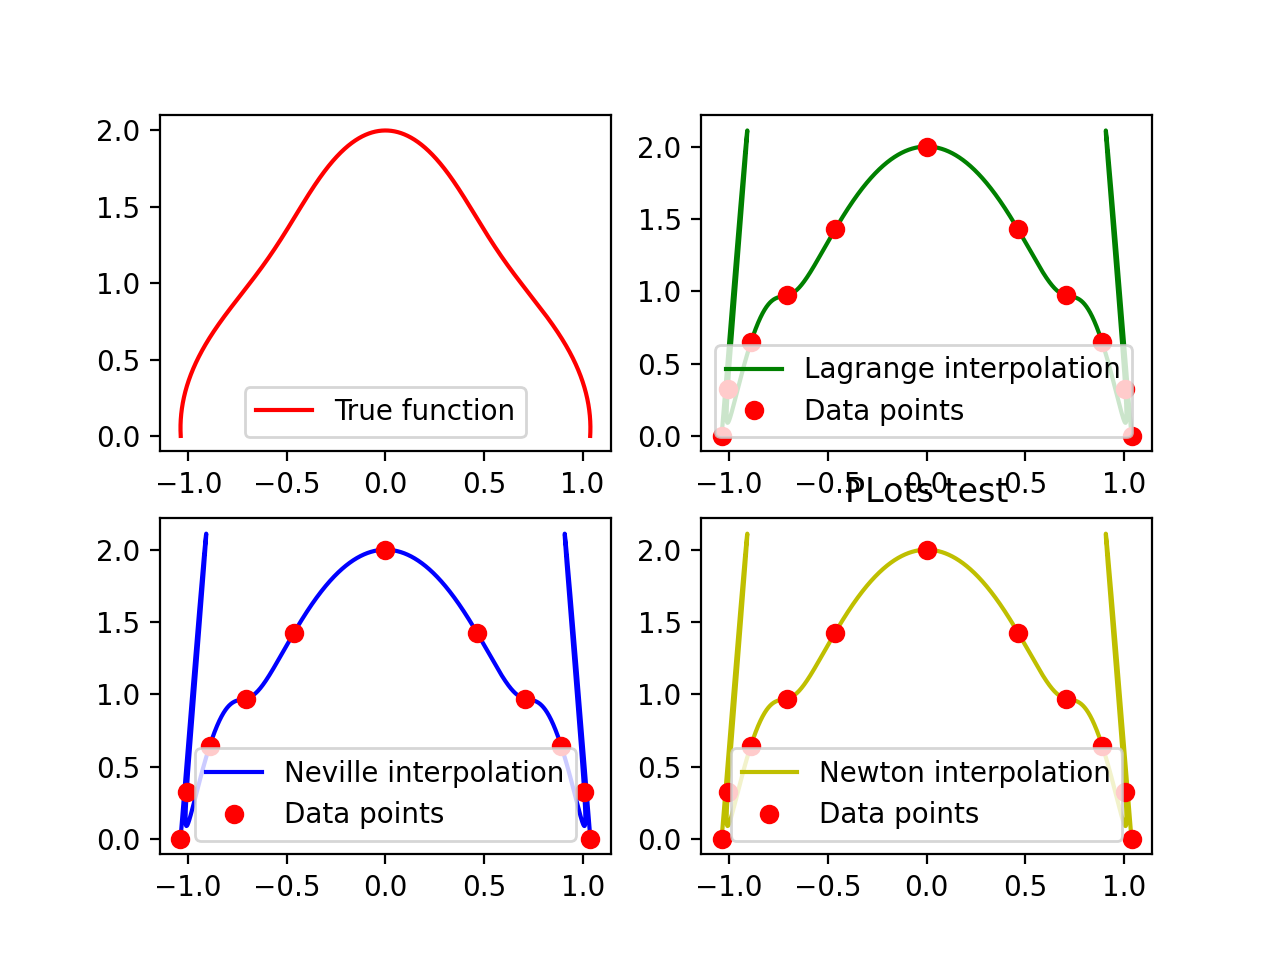
\includegraphics[width=0.7\columnwidth]{n=10}
	\caption{The 3 polynomials for n=10}
\end{figure}

For $n=20$ Neville took 5.022 seconds, Barycentric took 0.66 seconds and Newton took 0.49 seconds. \\

\begin{figure}[h!]
	\centering
	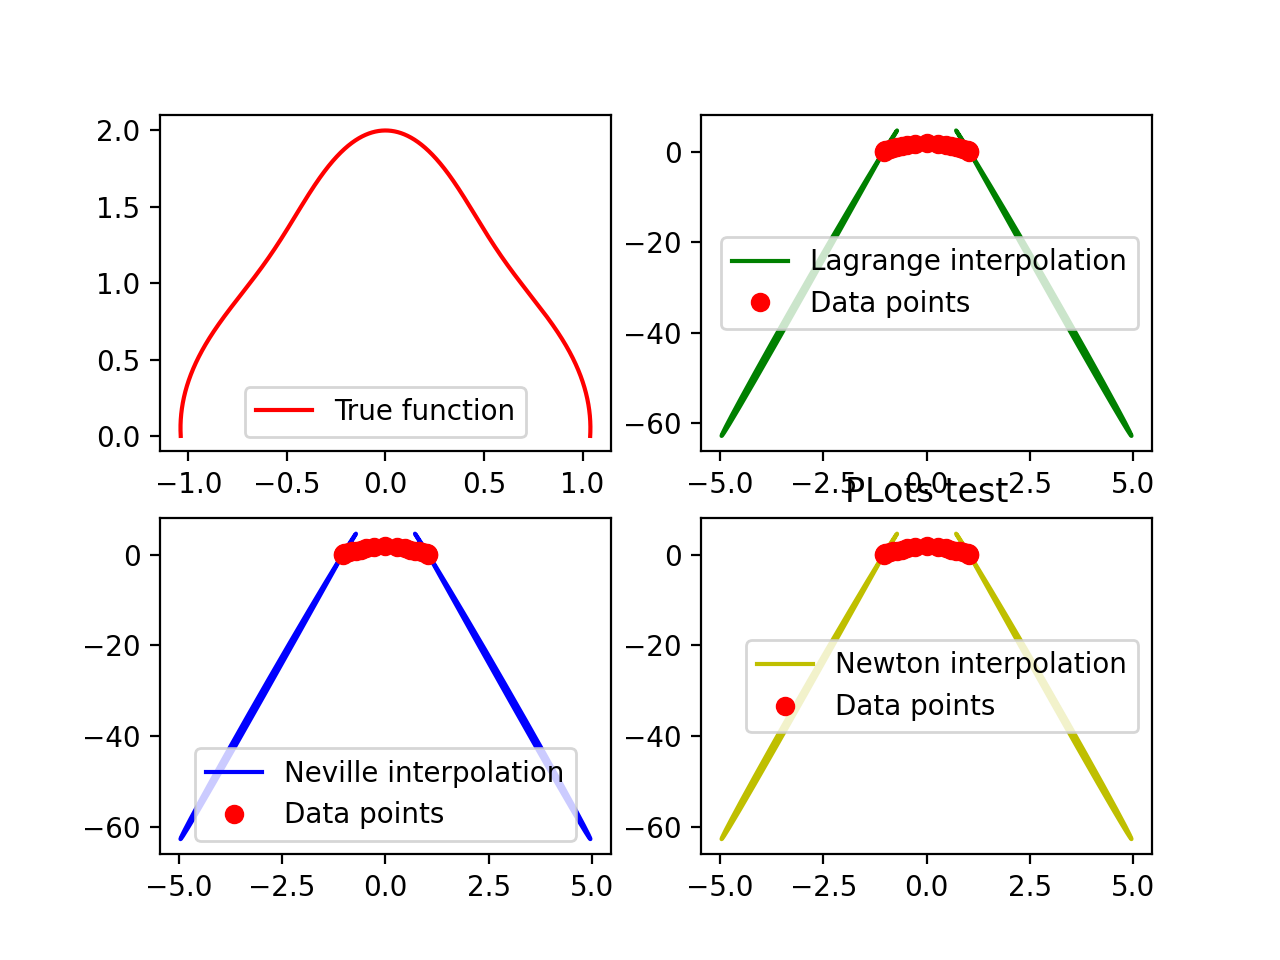
\includegraphics[width=0.7\columnwidth]{n=20}
	\caption{The 3 polynomials for n=20}
\end{figure}


For $n=40$ Neville took 20.41 seconds, Barycentric took 1.39 seconds and Newton took 1.43 seconds. \\

\begin{figure}[h!]
	\centering
	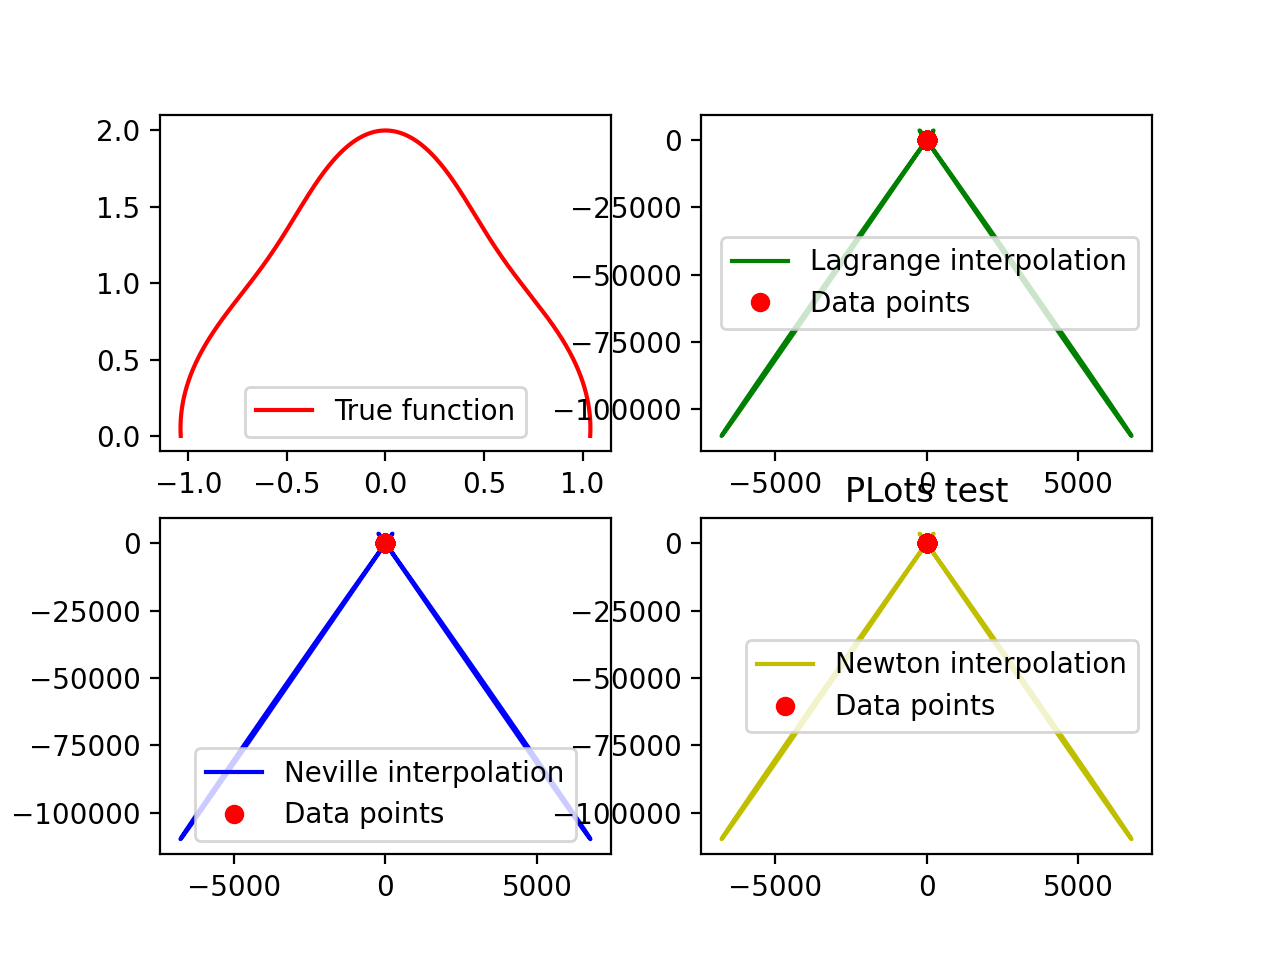
\includegraphics[width=0.7\columnwidth]{n=40}
	\caption{The 3 polynomials for n=40}
\end{figure}

By comparing the running time, Neville is by far the slowest, and Newton is slightly faster than Lagrangian. These results are according to the complexity theory of these 3 interpolation algorithms.\\

My plots clearly reveal that all my interpolation polynomials behave poorly in the proximity of the left and right boundary. However, by zooming in, each polynomial goes through the interpolation points. I didn't manage to solve this problem. Initially, I thought it was a stability problem but this is contradicted by the fact that Lagrange interpolation in barycentric form is a stable algorithm and therefore the results should be different from the two other algorithms. Probably I made some error(s) in my implementation. \\

\begin{figure}[h!]
	\centering
	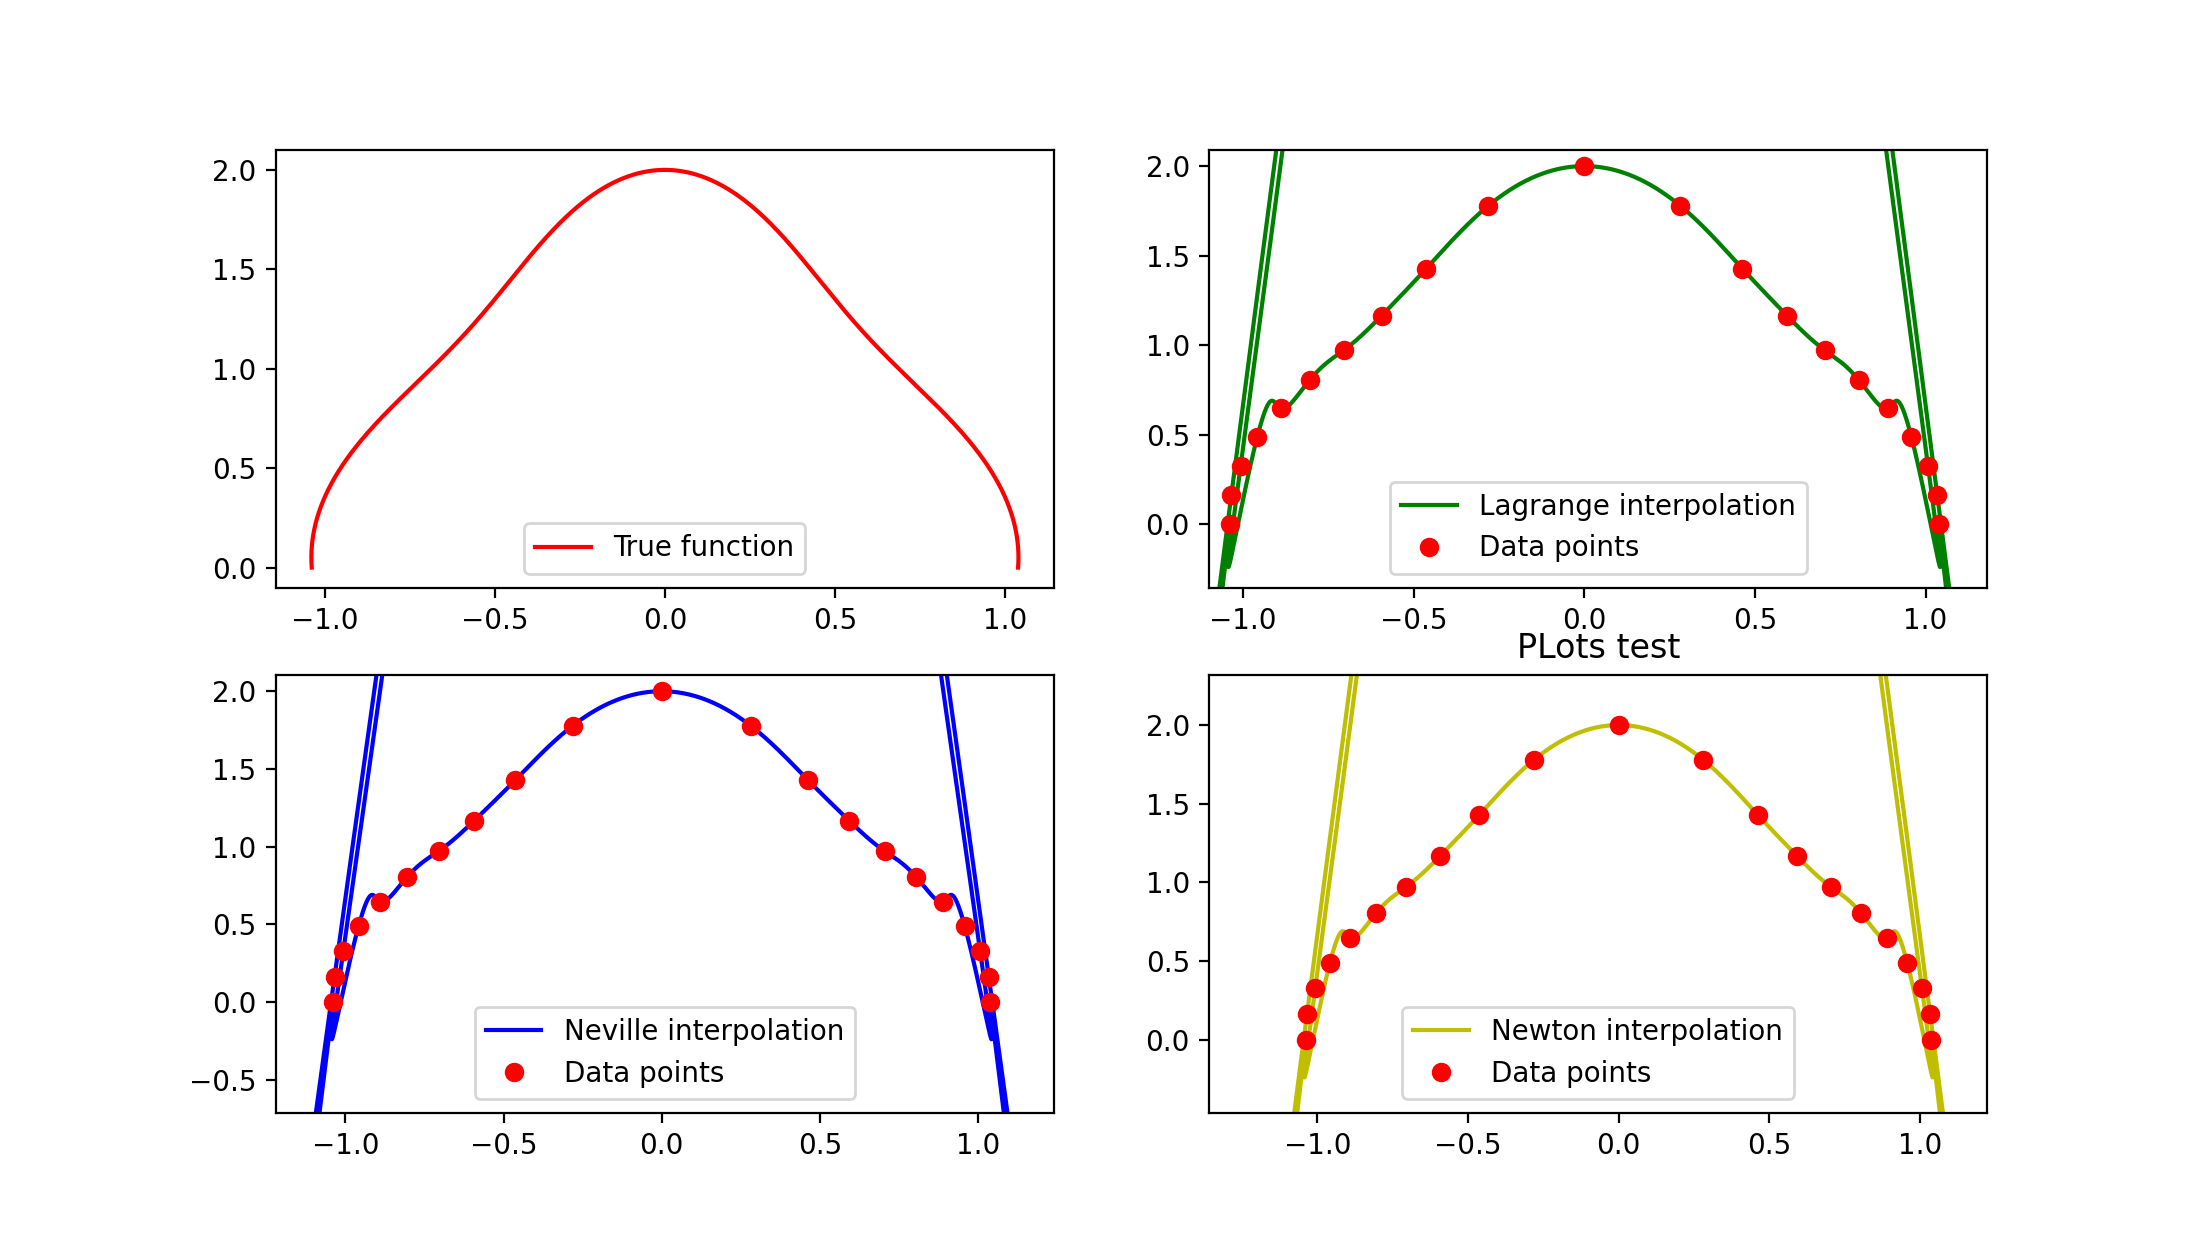
\includegraphics[width=0.7\columnwidth]{zoomin_n=20}
	\caption{Zoom in for n=20}
\end{figure}

\begin{figure}[h!]
	\centering
	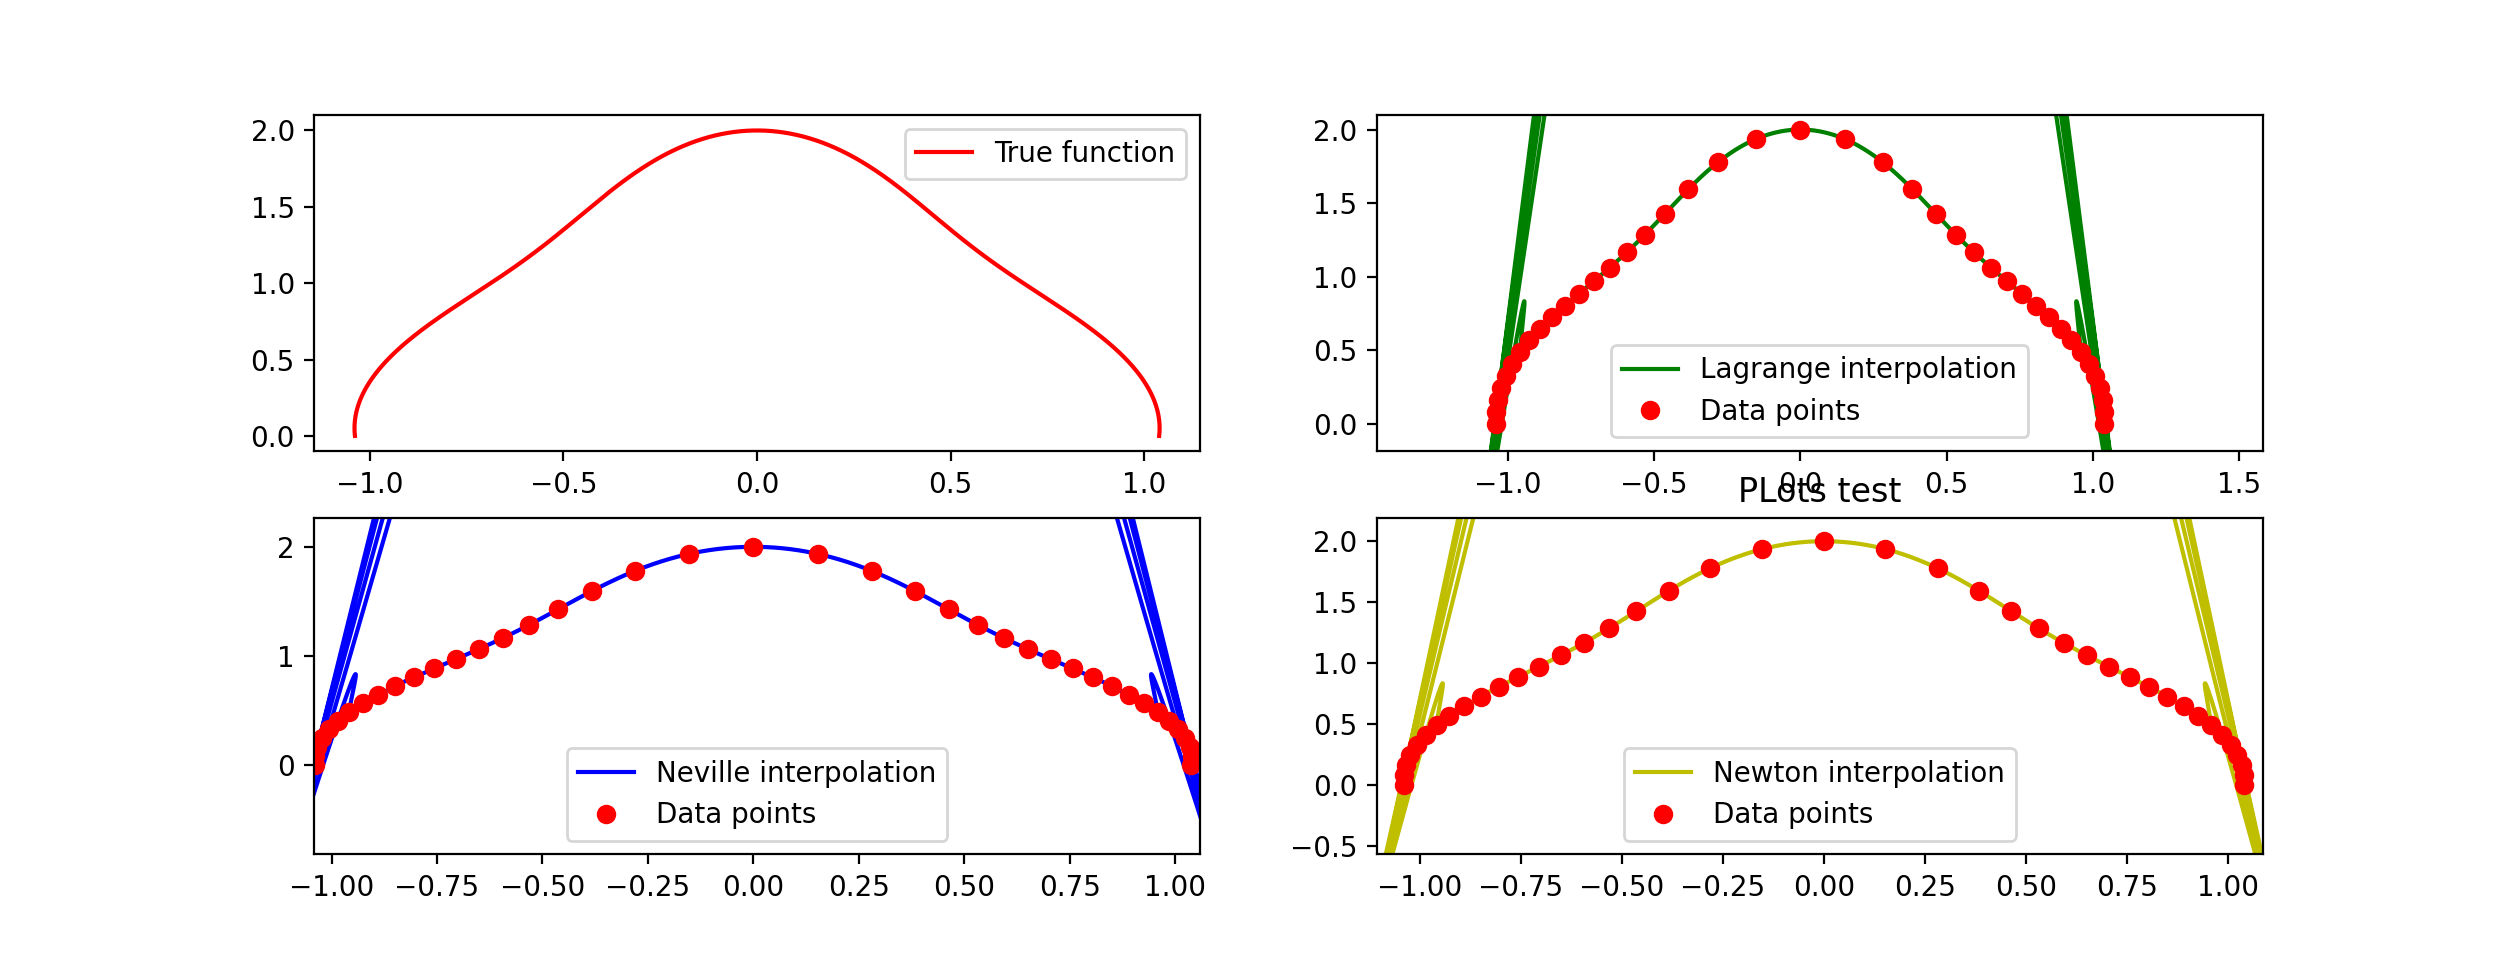
\includegraphics[width=0.7\columnwidth]{zoomin_n=40}
	\caption{Zoom in for n=40}
\end{figure}


\end{document}